\documentclass{article}
\usepackage[left=2.5cm, right=2.5cm, top=2cm]{geometry} 
\usepackage{graphicx}
%\documentclass[a4paper,10pt]{scrartcl}

\usepackage[utf8]{inputenc}

\title{Programa de Aula: Samba de Gafieira - Nível II}
\author{Fernando Pujaico Rivera}
\date{}

\pdfinfo{%
  /Title    (Sílabus: Samba de Gafieira - Nível II )
  /Author   (Fernando Pujaico Rivera)
  /Creator  ()
  /Producer ()
  /Subject  ()
  /Keywords (Samba, Gafieira)
}


\begin{document}
{\let\newpage\relax\maketitle}
A Tabela \ref{tab:typospos} e \ref {tab:typosmov}, descrevem a notação de nomes  (posturas e movimentos) usadas 
na descrição do programa de aula.
A Figura \ref{fig:mov} mostra como são relacionados as posturas e os distintos tipos de movimentos.


\begin{table}[h]
\centering
\begin{tabular}{|p{3cm}|p{13cm}|}
\hline
~ & Descrição \\  \hline
Postura & No transcurso das aulas, chamaremos postura o pose, a una distribuição estática
dos membros do corpo. Uma postura estabelece um ponto de inicio para a execução de um
movimento; assim, um movimento inicia e termina sempre numa postura o pose.\\ \hline

\end{tabular}
\caption{Descrição de uma postura}
\label{tab:typospos}
\end{table}


\begin{table}[h]
\centering
\begin{tabular}{|p{2.5cm}|p{13.5cm}|}
\hline
~ & Descrição \\  \hline
\textbf{Movimento} & É chamado como movimento ou ação, a um conjunto de trocas de peso ou deslocamentos de membros.
Um movimento não necessariamente tem um nome própio, se tiver, neste documento este será
chamado como passo.\\ \hline
\textbf{Transição ou movimento de transição} &  Movimento extremadamente simples, pelo qual geralmente não tem nome própio,
e constam de poucas trocas de peso e deslocamentos de membros. Exemplo: transição entre Frente trás e o Balanço, 
ou a transição entre Balanço e o Cruzado. Algumas transições
pelo seu uso na samba de gafieira, tem ganhado um nome própio, estes são: Saída lateral e Gancho.\\ \hline
\textbf{Passo (básico)} & Movimento de nível iniciante; o conhecimento deste tipo de
movimentos é necessário para enlaçar/interconectar movimentos mais complexos ensinados nas aulas. Estes
movimentos tem uma característica cíclica, é dizer, a postura do final do movimento 
é igual à postura de inicio. Os passos básicos são: Frente e trás (F.T.), Balanço e Cruzado.\\ \hline
\textbf{Passo} &  Movimento genérico com uma amplitude de dificuldade desde simples ate complexo.
Um passo inicia e termina numa postura, a qual pode ser a mesma. Definiremos como passo, a um movimento
notável, de modo que este tem ganhado um nome própio; exemplo: Gatilho, Gancho redondo, Romário, Puladinho, Elástico, etc. \\ \hline

\end{tabular}
\caption{Tipos de movimentos.}
\label{tab:typosmov}
\end{table}



\begin{figure}[h]
  \centering
  \caption{ Movimento sendo executado desde uma postura ate outra postura.}
  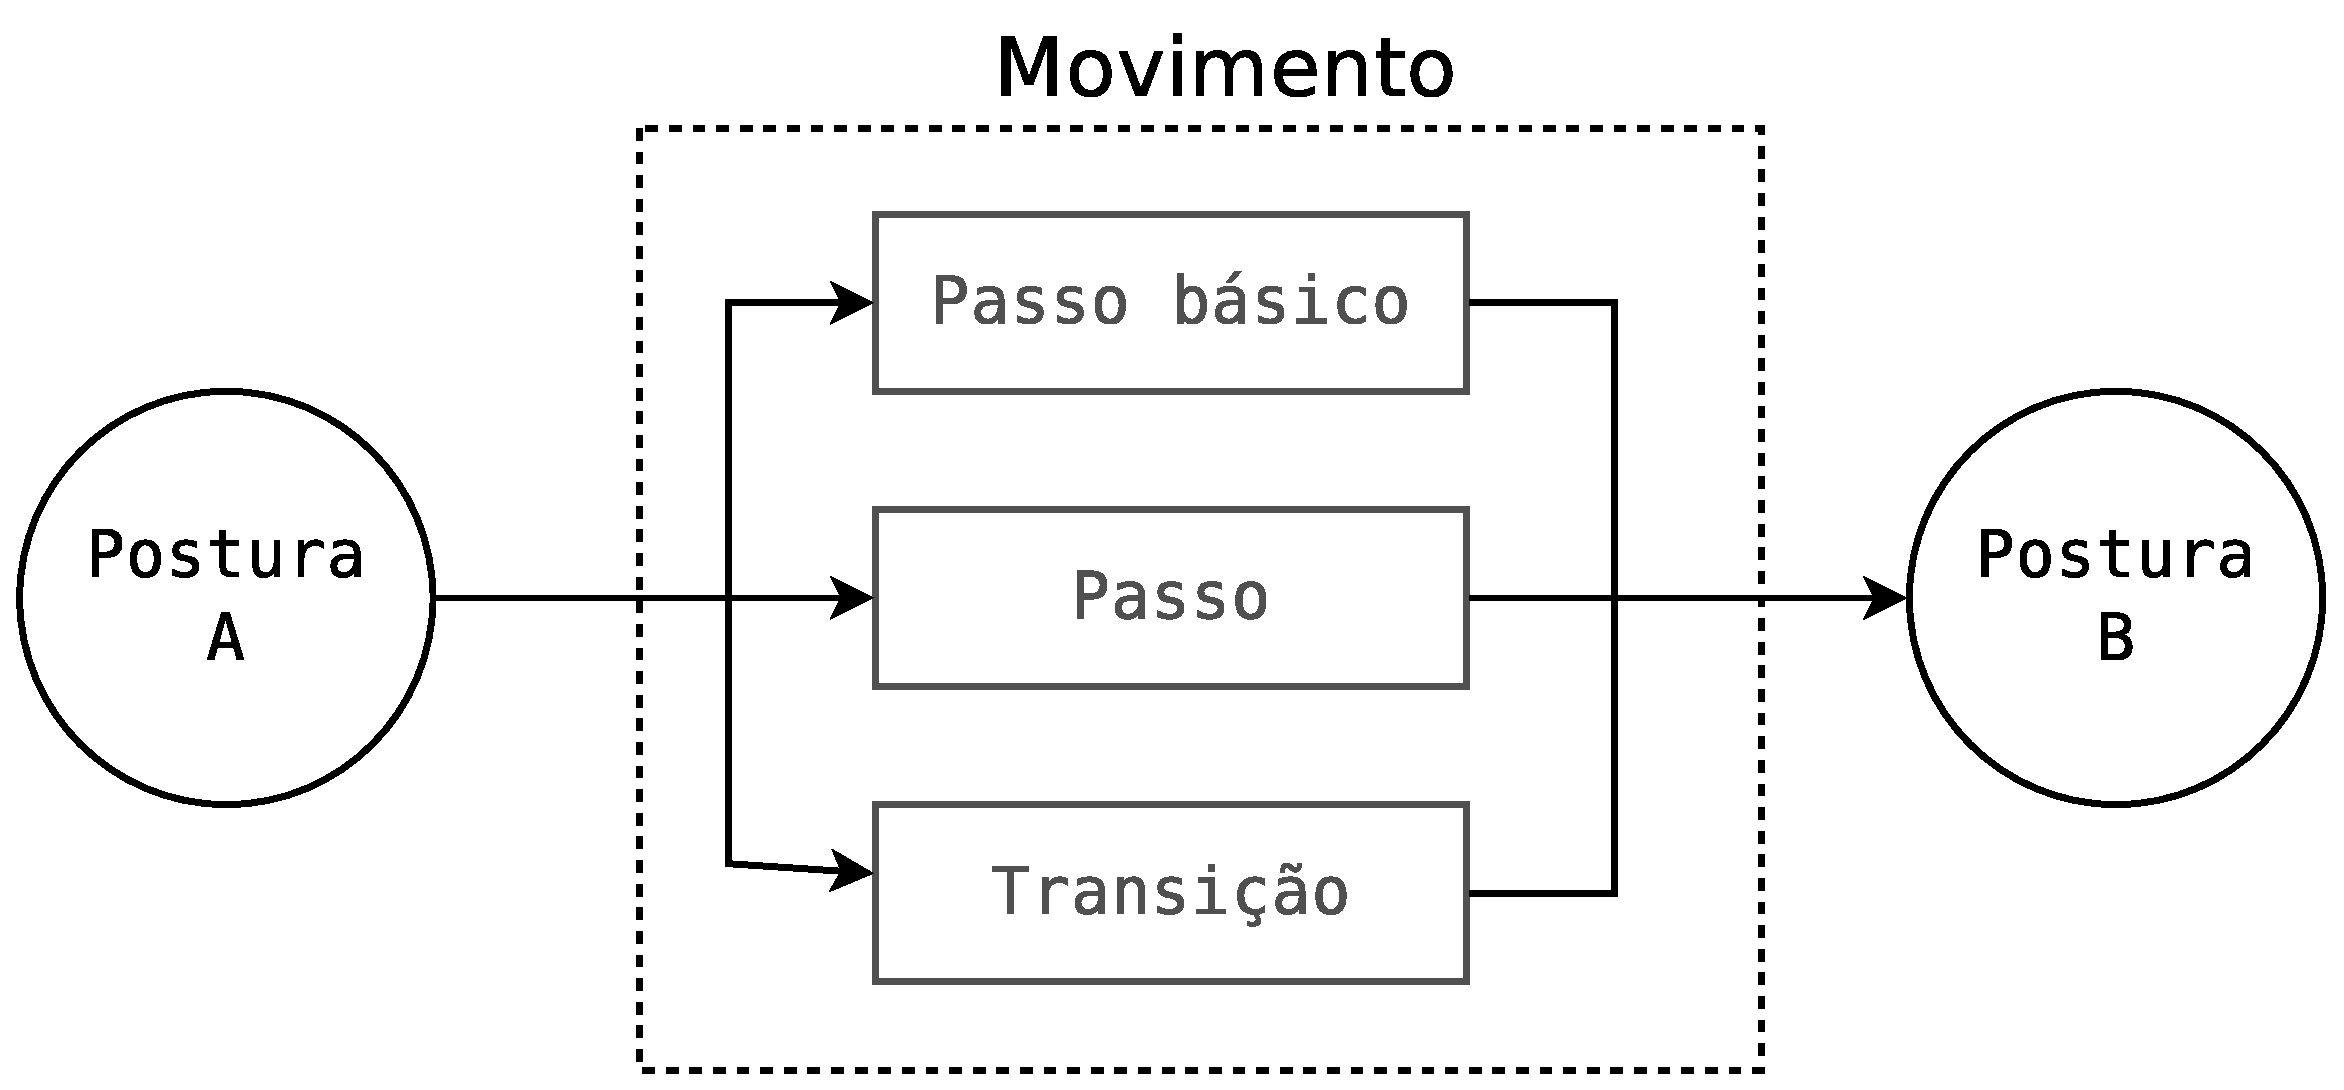
\includegraphics[width=0.8\textwidth]{Diagrama1.eps}% picture filename
  \label{fig:mov}
\end{figure}



A Tabela \ref{tab:myfirsttable} mostra a descrição do conteúdo das aulas de samba de gafieira.


\begin{table}[h]
\centering
\begin{tabular}{|p{1.5cm}|p{5cm}|p{9cm}|}
\hline
Semana & Tema & Descrição \\  \hline \hline
1 &  \textbf{Passo:} Frente e trás (F.T.), Balanço e Cruzado. &  Repasso do Frente e trás (F.T.), Balanço e Cruzado.\\ \hline
2 &  \textbf{Passo:} Balança corre corre. &  Repasso da saída lateral; e estudo do passo Balança corre corre.\\ \hline
3 &  \textbf{Passo:} Gancho redondo. &  Repasso do gancho; entradas e saídas do gancho redondo.\\ \hline
4 &  \textbf{Passo:} Puladinho &Entradas e saídas do movimento, e exercícios de consciência corporal para o quadril.\\ \hline \hline
5 &  \textbf{Passo:} Gatilho interrompido. &  Repasso do passo Gatilho; e estudo do passo Gatilho interrompido + enfeites.\\ \hline
6 &  \textbf{Passo:} Bailarina. &  Repasso do passo assalto; e diferencias com a bailarina.\\ \hline
7 &  \textbf{Passo:} Assalto interrompido. &  Repasso do passo assalto; e estudo do passo Assalto interrompido.\\ \hline
8 &  \textbf{Passo:} Trança. &  Repasso do balanço e saída lateral; estudo da trança.\\ \hline \hline
9 &  \textbf{Passo:} Picadilho. &  Estudo da condução e tempos do movimento.\\ \hline
10&  \textbf{Passo:} Romário com twist &  Repasso do passo Romário e estudo da inclusão de um twist pra remplazar o chute da moça. \\ \hline
11&  \textbf{Passo:} Facão invertido, \textbf{Postura}: Facão invertido. & Saída do facão invertido com sacada de perna. \\ \hline
12&  \textbf{Movimento:} Facão invertido + escovinhas. & Entradas e saída com escovinhas do facão invertido . \\ \hline \hline
13&  \textbf{Passo:} Elástico. &  Primeira aproximação ao movimento e se mostrarão algumas variantes.\\ \hline
14&  \textbf{Passo:} Pião. &  Primeira aproximação ao movimento, entradas e saídas.\\ \hline

%15&  \textbf{Passo:} Puladinho & Será estudado a consciência corporal necessária para executar o movimento, adicionalmente será agregado um enfeite para o movimento. \\ \hline

\end{tabular}
\caption{Descrição do conteúdo}
\label{tab:myfirsttable}
\end{table}

\end{document}
